\documentclass[tudarticle,type=msc,colorback,accentcolor=tud9c]{tudthesis}

  \usepackage[utf8]{inputenc}
  \usepackage[thmmarks]{ntheorem}
  \usepackage{xspace,cleveref,xcolor}
  \usepackage{amsmath}
  \usepackage{graphicx,url}
  \usepackage[font=small]{caption}
 \usepackage{subcaption}

% new commands
  \newcommand{\QQ}{\mathbb Q}
  \newcommand{\RR}{\mathbb R}
  \newcommand{\CC}{\mathbb C}
  \newcommand{\NN}{\mathbb N}
  \newcommand{\ZZ}{\mathbb Z}
  \newcommand{\DD}{\mathbb D}
  \newcommand{\A}{\mathcal A}
  \newcommand{\B}{\mathcal B}
  \newcommand{\C}{\mathcal C}
  \newcommand{\D}{\mathcal D}
  \newcommand{\R}{\mathcal R}
  \newcommand{\M}{\mathcal M}
  \newcommand{\laplace}{\operatorname\Delta}
  \bibliographystyle{plain}

  \newcommand{\p}{\ensuremath{\mathcal P}\xspace}
  \newcommand{\np}{\ensuremath{\mathcal{NP}}\xspace}
  \newcommand{\fp}{\ensuremath{\mathcal{FP}}\xspace}
  \newcommand{\abs}[1]{\left|#1\right|}
  \newcommand{\sharpp}{\ensuremath{\# \mathcal{P}}\xspace}
  \newcommand{\code}{\texttt}
  \newcommand{\cc}{\code{C++}\xspace}
  \newcommand{\irram}{\code{iRRAM}\xspace}
  \newcommand{\MPFR}{\code{MPFR}\xspace}
  \newcommand{\baana}{\code{BA\_ANA}\xspace}
  \newcommand{\anarect}{\code{ANA\_RECT}\xspace}
  \newcommand{\powerseries}{\code{POWERSERIES}\xspace}
  \newcommand{\real}{\code{REAL}\xspace}
  \newcommand{\temp}{\textcolor{red}}
  \newcommand{\seq}{\mathbf}
  \DeclareMathOperator{\lb}{lb}
  \DeclareMathOperator{\bigo}{O}
  \newcommand{\sprec}{prec\xspace}
  \newcommand{\demph}{\textbf}
  \newcommand{\sdzero}{\texttt{0}}
% ntheorem environments
  \theoremseparator{:}
  \theorembodyfont{\itshape}
  \newtheorem{definition}{Definition}
  \theorembodyfont{\upshape}
  \newtheorem{theorem}[definition]{Theorem}
  \newtheorem{corollary}[definition]{Corollary}
  \newtheorem{example}{Example}[section]
  \newenvironment{proof}{\paragraph{Proof:}}{\hfill$\square$}
\begin{document}
  \thesistitle{Case Studies in Exact Real Arithmetic - Implementations and empirical Evaluation}{Fallstudien in exakter reeller Arithmetik: Implementation und empirische Evaluation}
  \author{Holger Thies}
  \referee{Prof. Dr. Martin Ziegler}{tba}[tba]
  \department{Mathematics}
  \group{Mathematical Logic}
  \dateofexam{\today}{\today}
  \makethesistitle
  \affidavit{H. Thies}
\dedication{Danksagung...}
\begin{abstract}
    Abstract...
\end{abstract}  
\tableofcontents
  \chapter{Introduction}

  \chapter{Theoretical Background}
  \section{Floating Point Arithmetic and Real Numbers}
  %!TEX root = ../../thesis.tex
\section{Real Computability Theory}\label{sec:real computability}
\subsection{Classical Computability Theory}
 Since in real computability theory many aspects of classical computability theory are extended, 
 a very brief overview is given in the following section.

 To define computability the Turing-Machine model is used.
 The Turing-Machine was invented by Alan Turing in 1936 \cite{Turing} and can
 be seen as simplified mathematical model for a computer.

 The machine constists of an infinite tape that is divided into cells. 
 Each cell contains exactly one symbol from a predefined finite alphabet
 $\Sigma$.
 It further consists of a head that is always positioned on top of one cell 
 and can in one step read and write the content of the cell and then move one
 cell left or right on the tape.

 The machine is always in one of finitely many states and has a finite
 instruction table containing instructions of the form when in state $q$ and
 reading symbol $s$, write $s'$ and move head to the left (or to the right).

 A formal definition can for example be found in \cite{Hopmann}.
 
 \begin{definition}
 	A possibly partial function $f:\subseteq \Sigma^* \to \Sigma^*$ is called \textbf{computable} if there exists 
 	a Turing-Machine, so that for all $x \in dom(f)$ the machine terminates after finitely many steps with $f(x)$ on its 
 	tape and for $x \not \in dom(f)$ the machine does not terminate.
 \end{definition}

 Even tough the Turing-Machine model is quite simple, it can be used to
 simulate every computer algorithm.
 The widely believed \textbf{Church-Turing thesis} even states, that anything
 that is computable in an informal sense, can be computed with a
 Turing=machine.

 The following definitions for sets also play a very important role in
 computability theory:
 \begin{definition}
 	A set $A \subseteq \Sigma^*$ is called \textbf{decidable}, if its characteristic function is computable. 
 \end{definition}
 \begin{definition}
 	A set $A \subseteq \Sigma^*$ is called \textbf{recursively enumerable} (r.e.) or \textbf{computably enumerable} (c.e.) if 
 	it is empty or if $A$ is the domain of a computable function.   
 \end{definition}
\subsection{Computability of real numbers}
The previous section showed how to define computability over finite alphabets $\Sigma^* \to \Sigma^*$. 
That is enough to define computability for finite structures. The following section defines how to extend 
the classical notion to uncountable objects such as real or complex numbers, functions or infinite sequences.
There are several non equivalent ways, to define computability on such objects. 
In contrast to the classical case, where the definition given in the previous section is widely accepted, there is no 
generally accepted model for real complexity theory.

The model used in this thesis is the so called \textbf{Type 2 Theory of Effectivity} (TTE). 
Because... 

This section gives an overview of the framework used to define computability on real numbers and is therefore 
a little more general then needed in the rest of the thesis, that focuses more on implementations of subsets of this framework.
However,...

The general definition is by Type-2 Turing Machines...
From now on the term Turing-Machine is used both for classical and type 2 machines, when it is clear by context which model is meant.
\begin{definition}\label{def:computability_ttt}
A function $F:\subseteq \Sigma^\omega \to \Sigma^\omega$ is called computable if there is a Turing-Machine  
that for all infinite strings $\sigma in dom(F)$ writes the infinite string $F(\sigma)$ on its output tape. 
For $\sigma \not \in dom(f)$ the machine writes only finitely many symbols on the output tape.  
\end{definition}
To talk about computability over some set, the notion of encoding this set to $\sigma^\omega$ has to be formalized.
\begin{definition}\label{def:representation}
	A \textbf{representation} of a set $X$ is a partial surjective mapping $\alpha: \sigma^\omega \to X$. \\
	$\bar \sigma \in \alpha^{-1}(\sigma)$ is called an \textbf{$\alpha$-name} of $\sigma$. \\
	$x \in X$ is \textbf{$\alpha$-computable} if it has a decidable $\alpha$-name.
\end{definition}

Of course, the definition of representations is open wide and can lead to many different more or less useful definitions of computability.
Some possible representations for real numbers are as follows
\begin{enumerate}
\item A $\rho_{10}$-name of $x$ is the usual decimal expansion of $x$.
\item A $\rho$-name of $x \in \RR$ is a sequence $a_n \in \ZZ$ s.t. $| x - a_n | \leq 2^{-n}$
\item  A $\rho_C$-name of $x \in \RR$ consists of two sequences rational $(q_n)_{n \in \NN}$ and $(\varepsilon_n)_{n \in \NN}$, so that 
$| x_n - q_n | < \varepsilon_n$ and $\lim_{n \to \infty} \varepsilon_n = 0$  
\item $\rho_<$-name, $\rho_>$-name
\item $\rho_n$-name 
\end{enumerate}
\begin{theorem}
The following are equivalent
\item $x \in \RR$ is computable in the sense of Definiton 
\item $x \in \RR$ is $\rho_{10}$ computable
\item $x \in \RR$ is $\rho$-computable
\end{theorem}
\begin{example}
Specker-Sequence
\begin{definition}\label{def:representation_composition}
Composition of representations
\end{definition}
\end{example}
This thesis does not deal with the problem of computing single real numbers, but rather with computing real functions and real functionals.
For a function $f:\subseteq \RR \to \RR$ to be computable means, that is it possible to compute $f(x)$ arbitrarily good. 
Also a machine can not read $x$ with infinite precision, but it can ask to get $x$ as exact as it needs it to compute the output.
\begin{definition}\label{def:computability_oracle_tm}
\end{definition}
This concept can be generalized by the following definiton  
\begin{definition}\label{def:computability_function_representation}
	A function $f: \subseteq X \to Y$ is called \textbf{$(\alpha, \beta)$}-computable, 
	if there exists a computable function $F:\subseteq \Sigma^\omega \to \Sigma^\omega$ such that 
	$\beta(F(\sigma)) \in f(\alpha(\sigma))$ for all $\sigma \in dom(f \circ \alpha) $.  
\end{definition}
The Diagram in ... shows computability.
Examples...
\begin{theorem}
Multiplication is not $(\rho_{10}, \rho_{10})$-computable.
\end{theorem}
From now on the term computable will be used to describe computability w.r.t. the Cauchy representation.
Then all of the following functions are computable
\begin{enumerate}
\item Arithmetical operations $+,-,x,/ : \subseteq \RR^2 \to \RR$
\item The absolute value function
\item The minimum and maximum functions
\item constant functions with computable constant
\item Projections $\RR^k \to \RR$ 
\item polynomials with computable coefficients
\item $exp, sin, cos$
\item The square-root function and the logarithm function
\end{enumerate}
\begin{theorem}
	Computable functions are continuous...
\end{theorem}

\begin{theorem}
Computability is preserved under function composition, i.e.
For sets $X,Y,Z$ with representations $\delta_X, \delta_Y, \delta_Z$, 
$f:\subseteq X \to Y$ $(\delta_X, \delta_Y)$-computable and $g:\subseteq Y \to Z$ $(\delta_Y, \delta_Z)$-computable,
$g \circ f$ is $(\delta_X, \delta_Z)$-computable.
\end{theorem}
\begin{definition}
A multi-valued function $f: \subseteq X \rightrightarrows Y$ is just an other name for a relation $f \subseteq X \times Y$.
A multi-valued function is $(\rho_X, \rho_Y)$ computable, if there is a a comnputable (single valued) function 
$F: \subseteq \Sigma^\omega \to \Sigma^\omega$ such that for all $\sigma \in dom(f \circ \rho_X)$, $\rho_Y(F(\sigma)) \in f(\rho_X(\sigma))$. 
\end{definition}
\subsection{Computability of real operators and functionals}
A real operator maps functions $\RR \to \RR$ to functions $\RR \to \RR$and a functional maps functions $\RR \to \RR$ to real numbers $\RR$.
For that, a representation for the space to work on is needed.
Continuous functions on a compact subset $X \subseteq R^d$ can be uniformly approximated by polynomials arbitrarily close.
A possible representation for real valued functions is thus given by the following definition 
\begin{definition}
A $[\rho^d \to \rho]$-name of a function $f \in C([0,1]^d, \\R)$ is given by a sequence $P_n \in \\D[x1, \dots, x_d]$ of polnomials (i.e. degree and list of coefficients), such that $\vert f - P_n \vert_\infty < 2^{-n}$   
\begin{theorem}[name?]
The integration operator 
$$I: C[0,1] \ to C[0,1], f \to (x \to \int_0^x f(t) dt$$   
is computable.
\end{theorem}
\begin{theorem}[Myhill 1971]
There is a computable function $f: [0,1] \to \R$ with continuous but uncomputable derivative. 
\end{theorem}
\begin{theorem}
The operator 
$$ D: C^1[0,1] \to C[0,1], f \to f'$$
is computable.
\end{theorem}
\end{definition}
\subsection{Uniformity and Non-Uniformity}
When talking about computability one has to distinguish between two types of computability, \textbf{uniform} and \textbf{non-uniform}.
FOr non-uniform computability it suffices, that for every input, there is an algorithm that computes the output. 
The algorithm may however depend on the input in a non-computable way.
In contrast, a problem is uniformly computable only if there is one algorithm, that computes the output for every valid input. 
Intermediate Value Theorem
\subsection{Other models for comoutable reals}
Markov Computability \\ 
Sequential Computabilty \\
Computable invariance \\
BSS-model \\

  %!TEX root = ../../thesis.tex
\section{Real Complexity Theory}\label{section:real_complexity}
	\subsection{Classical Complexity Theory}
    In contrast to computability theory, complexity theory deals with the
    question how many resources (in form of e.g. time or space) are needed to
    compute a computable function.

    Again, the Turing-Machine model is used to describe the computations
		\begin{definition}
			For a given Turing Machine $M$ and $w \in \Sigma^*$, $time_M(w)$ is the number of head movements 
			the Turing Machine on input $w$ exectues before it terminates. \\
			For $n \in \NN$ define $time_M(n) = \max \{ time_M(w) \,|\, w \in \Sigma^* and M terminates on input w \}$.\\
			Analogously, one can define space constraints.
		\end{definition}
    In most cases it is not important to compute the exact running time, but
    one rather wants to approximate how the algorithm will behave when the
    input is getting large.
    The standard way to compare the asymptotic running time of algorithms is
    the use of $O$-notation.
		\begin{definition}
			For functions $f, g: \NN \to \NN$ one writes $f \in O(g(n))$ if there are constants $M \in \RR$, $n_0 \in \NN$, such that
			$ f(n) \leq M \cdot g(n)$ for all $n > n_0$. 
		\end{definition}
			Thus, for a given algorithm a way to measure its complexity is giving an
      upper bound on its worst case running time for inputs of length $n$ in
      terms of the $O$-notation. 

			However, complexity theory mainly is not about the complexity of specific
      algorithms, but rather deals with the complexity of problems. 
      That is, trying to classify the complexity of \textbf{any} algorithm to
      decide a subset of $\Sigma^*$.
      
      The following gives a classifications of problems depending on the
      running time for algorithms solving those problems.
		\begin{definition}
			For a function $t: \NN \to \NN$ let 
      $$ \text{DTIME}(t) = \{ A \subseteq \Sigma^* \,|\, \text{There is a
      Turingmachine } M \text{ deciding } A \text{ with time}_M(n) \in O(t(n)) \} $$

      NTIME$(t)$ describes the same for the case of $M$ being a
      non-deterministic Turing-machine.
		\end{definition}
		The above definitions suffice to define the most important complexity classes
		\begin{definition}
			The complexity classes $P, NP, PSPACE$ and $EXPTIME$ are defined as follows:
			\begin{eqnarray*}
				P & := & \bigcup_{k \in N} DTIME(n^k) \\
				NP & := & \bigcup_{k \in N} NTIME(n^k) \\
				PSPACE & := & \bigcup_{n \in N} DSPACE(n^k) \\
				EXPTIME & := & \bigcup_{k \in N} DTIME(2^{n^k}) \\
			\end{eqnarray*}
		\end{definition}
		It holds $P \subseteq NP \subseteq PSPACE \subseteq EXPTIME$. 
		It is $P \neq EXPTIME$ and for all other inclusions it is not known if equality holds, but most 
		complexity theorists consider it as extremely unlikely.

    Another way to characterize the important class $NP$ is the following
    \begin{theorem}
      $A \subseteq \Sigma^*$ is in $NP$ if and only if there are polynomials
      $p$ and $q$ and a deterministic Turing-Machine $M$ such that for all $x
      \in \Sigma^*$ with length n, there is an $y \in \Sigma*$ with length
      bounded by $q(n)$ such that $x \in A \text{ iff } M(<x,y>) = 1$ and 
      $x \not \in A \text{ iff } M(<x,y>) = 0$. 
      Further $M$'s running time is bounded by $p(n)$ for all such inputs
      $<x,y>$.  
    \end{theorem}
		Wheter $P = NP$ is one of the Millenium problems and one of the biggest unsolved problems in Computer Science.

		One can also consider function problems instead of decision problems
    leading to a dual hierarchy of complexity classes.
		\begin{definition}
      A functional problem $F: \Sigma^* \rightrightarrows \Sigma^*$, is solved
      by a Turing-Machine in if it writes on every $x \in \Sigma^*$ an output
      $z \in F(x)$ or decides that no such output exists.  \\ Time- and
      Space-Complexity can be defined accordingly. \\ The classes $FP$ and
      $FPSPACE$ are defined as the class of polynomial time resp. space
      computable functions. \\ The class $\#P$ is defined as the the class of
      functions that give the number of solutions to a problem in $NP$.
    \end{definition}
		It holds $FP \subseteq \#P \subseteq FPSPACE$ and if $FP = \#P$ would hold, it would follow that $P = NP$.
     
		Problems that are known to be in $P$ are often considered as the feasible functions, 
		for which it is possible to find an efficient algorithm. 

    Since most of the complexity classes are not known to be distinct, they do
    not suffice to classify problems by their difficulty.
    To compare the difficulty of problems, reductions are used.
		\begin{definition}
			$A \subset \Sigma^*$ is \textbf{polynomial time reducible} to $B \subseteq \Sigma^*$ ($A \leq_P B)$, 
			if there is a polynomial time computable function $f; \Sigma^* \to \Sigma^*$, such that
			$$ w \in A \Leftrightarrow f(w) \in B.$$
		\end{definition}
		Many other types of reductions exist, e.g. to compare complexity classes
    lower then $P$, but they are not needed in this thesis and therefore
    omitted.

		The hardest problems in a complexity class are called complete for this class
		\begin{definition}
			A set $A \subseteq \Sigma^*$ is called \textbf{$\C$-hard} (w.r.t. $\leq_P$) for a complexity class $\C$, if for all $B \in \C$ $B \leq_P A$. \\
			$A$ is called \textbf{$\C$-complete} (w.r.t. $\leq_P$), if $A$ is $\C-hard$ and $A \in \C$.  
		\end{definition}
		If one would show for a single $\C$-complete problem that it is in $P$, it would follow that all problems in $\C$ are in $P$.
		Consequently a way to show that there is most likely no efficient algorithm to a problem, is to show that the problem is $NP$-hard.
    For many problems it could be shown that they are $NP$-complete. 
    Some of the most important ones can for example be found in
    \cite{bookwithnpcompleteproblems}
	\subsection{Complexity Theory on real numbers}
		In classical complexity theory the time complexity is usually measured in terms of the input size.
		However, when considering continuous peoblems, the input is an infinite string and thus can not 
		be used to measure the running time of an algorithm.

		In numerical computations an important parameter is the desired output precision.
		Thus, it seems reasonable to analyze the running time as a function depending on the desired output precision.
    
		This leads to the following definition for the complexity of a single real
    number
		\begin{definition}\label{def:complexity_real_number}
			A real number $x \in \RR$ is computable in time $t$ if there is a Turing Machine $M$ that with input $n \in \NN$ in binary, 
			outputs the binary expansion of a dyadic rational number $d$ with $| x - d | \leq 2^{-n}$.  
		\end{definition}
		Again this notion can be generalized by using representations and type-2
    Turing machines, i.e. by considering the time that is needed to write the first $n$ symbols
		of the name of the output.
      
    One has to be careful, however, since representations that are
    computationally equivalent, do not necessary lead to the same complexity
    bounds.  For example, one can construct arbitrarily long Cauchy names for
    any rational number.
    Thus, it is not even possible to define the complexity of a real number
    with respect to its Cauchy name.

		A more useful representation for complexity is the signed-digit
    representation.
		\begin{definition}
			The \textbf{signed digit representation} $\rho_sd$ is defined as follows: 

			A $\rho_d$-name of a real number $x$ is a sequence 
			$$a_n a_{n-1} \dots a_0 . a_{-1} a_{-2} \dots \text{ with } a_i \in \{-1,0,1\}, n \geq -1, a_n \neq 0, a_n + a_{n-1} \neq 0$$
      and
			$$  x = \sum_{i=n}^{-\infty} a_i \cdot 2^i $$  
		\end{definition}
		As with the binary expansion, the number digits after the binary point correspond to the precision.

		\temp{The advantage to the binary expansion is that, the signed digit
    representation is symmetric, ,,,}
		It can be shown that the signed digit representation is computably equivalent to the Cauchy representation.

		When extending the complexity notion to functions, apart from the output
    precision, an additional parameter might be interesting: the precision of the input
		needed to compute the output up to the demanded precision.

    This leads to the following definition
		\begin{definition}
      A function $f: \subseteq \RR \to \RR$ is computed on a compact set $K
      \subseteq dom(f)$ in time $t$ with lookahead $l$ if for all
      $\rho_{sd}$-names of elements $ x \in K$ by a Turing Machine $M$ if $M$
      computes a $\rho_{sd}$-name of $f(x)$ and after t steps and with reading
      at most $l$ symbols of the input string outputs the $n$-th symbol of the
      output.   
    \end{definition} 
    The above comolexity notion really only makes sense on a compact set, since
    otherwise the machine could already spend arbitrarily much time on just
    reading the input left from the binary point.
    
    An alternative approach to define complexity of functions is using Oracle
    Turing Machines which have polynomial time bounded running time. 

    With the above notion computable real numbers and functions can be
    classified into complexity classes like in the discrete case.
    An important class for practical purposes is the class of polynomial time
    computable numbers and functions, since they usually can be computed
    efficiently with a computer.
   
    An important property of polynomial time computable reals is given in the
    following theorem.
		\begin{theorem}[Ko and Friedmann]
			The set of polynomial time computable real numbers forms a real algebraically closed field.
		\end{theorem}
		\begin{example}
     The following real valued functions are polynomial time computable on a compact set
     $K$
     \begin{enumerate}
       \item Addition, Subtraction and Multiplication as functions $K \times K
         \to \RR$.
        \item The function $x \mapsto \frac(1){x}$ if $0 \not in K$. 
         \item The functions $\exp, \sin, \cos$ as functions $K \to \RR$.
     \end{enumerate}
		\end{example}
	\subsection{Complexity of Operators}
		Since most interesting function spaces such as $C[0,1]$ are not locally compact,
		there is no straight forward way to generalize the above definitions to get
    a uniform notion of complexity for operators.

		In fact, the following holds
		\begin{theorem}
      Even restricted to continuous functions $f: [0,1] \to [0,1]$, the
      evaluation operator $x \to f(x)$ is not computable within time uniformly
      bounded in terms of the output error only.  
    \end{theorem}

	  A different approach to study the complexity of operators and functionals
    is followed by Ko and Friedman \cite{KoBook}.
    Instead of trying to define a complexity notion for a functional $F$, they
    study the time complexity of the real valued function $F(f)$ where $f$ is a
    polynomial time computable function.


		This  method leads to many connections between discrete complexity classes
    and numerical problems,

    One example of such a connection is given in the following theorem.
		\begin{theorem}[Friedman \cite{Fri}]
			The following are equivalent
			\begin{enumerate}
				\item $FP = \#P$
				\item For every polynomial time computable function $f: [0,1] \to \R$, the function
					$g: [0,1] \to \R$, defined by $g(x) = \int_0^x f(t) dt$ is polynomial time computable.
			\end{enumerate} 
		\end{theorem}
		Thus, one can say that integration of polynomial time computable functions is at
    least as hard as solving a problem in $\#P$.
    In that sense, Integration can be called $\#P$-hard.

    \temp{Maybe add something on second order representations}
 	\subsection{Parameterized Complexity}
  \temp{Write something or remove this section.}

  \chapter{iRRAM}
  \section{Real Number representation}
  \section{Overview of Classes}
  \section{Multivalued Functions}
  \section{Similiar Frameworks}

  \chapter{Case Studies}
  %!TEX root = ../../thesis.tex
\section{Dynamic Systems and the Shadowing Lemma}
\subsection{Introduction}
  \begin{definition}
    A \textbf{discrete dynamical system} is a triple $(\NN,X,\Phi)$ with $X$ a non empty set (the state space) and an operation $\Phi : \NN \times X \to X$, so that
    $\Phi(0,x) = x$ and $\Phi(n,\Phi(m,x)) = \Phi(n+m, x)$. 
    Thus, a discrete dynamical system is the model of a system, that evolves over discrete time steps.
  \end{definition}
  The simplest case of a discrete dynamical system, is when the state space is 1-dimensional (say $X \subseteq \RR$) and 
  the transition function only depends on the previous value, i.e. $\Phi(1,x) = f(x)$ for some $f : \RR \to \RR$. 
  Then the dynamical system can be written by the recurrence relation $x_{n+1} = f(x_n)$ with initial condition $x_0 \in \RR$.
  A chaotic system is a dynamical system, that is highly sensitive to initial conditions.
  A consequence of that is that even relatively small numerical errors in the computation grow exponentially fast.
  A prototypical example of a chaotic system is the logistic map:
  \begin{definition}\label{def:logmap}
    The \textbf{logistic map} is given by the recurrence relation 
    $ x_{n+1} = ax_n(1-x_n) \text{ with } a, x_0 \in \RR$.
  \end{definition} 
  \begin{table}
    \begin{tabular}{ | c | c | }
    \hline
    $a$ & behaviour \\ \hline
    $[0,1]$ & Stabilizes at $0$ \\ \hline
    $(1,3]$ & Stabilizes at $\frac{a-1}{r}$ \\ \hline 
    $(3, \approx 3.544]$ & oscillates between $2$, $4$, $8$, $\dots$ values. \\ \hline 
    $(\approx 3.544, 4]$ & \begin{tabular}{l}almost all inital points no oscillation with finite period \footnote{This is true for most points in this interval. There are however isolated ranges of $a$ for which the oscillation period is finite.}  \\ Small changes in the initial point yield large differences over the iterations. \end{tabular} \\ \hline
    $(4, \infty)$ & The values eventually leave the interval [0,1] and diverge for almost all initial points \\ 
    \hline
    \end{tabular}
    \caption{behaviour of iterating the logistic map for different values of the parameter $a$}\label{table:logmapbehaviour}
  \end{table}
  The logistic map behaves differently for different values of the parameter $a$ as can be seen in Table \ref{table:logmapbehaviour}. 
  The for this thesis interesting case is for $a \in (3.544, 4)$ where the iteration of the map leads to chaotic behaviour.

  Since the \irram framework can be used to compute iterations of the logistic map exactly, it is very well suited to invesitgate this chaotic behaviour \footnote{what could also be shown in a contest in 2000 \cite{competition:2001}}. 

  Figure \ref{fig:logmaperror1} shows how sensitive the map is to small errors that occur because of finite precision computations. 
  When using 10 significant digits for the computation, it can be seen that after around 50 iterations the finite precision version diverges from the \irram version and then behaves completely differently. 

  \irram can also be used to approximate the complexity in terms of needed computation precision. Since \irram automatically increases the internal precision until it suffices to output the result with the demanded number of digits, the internal precision at the end of the computation gives a measure of this complexity. As can be seen in Figure \ref{fig:logmapprec}, the needed internal precision grows extremely quickly with the number of iterations.
  To compute 10 significant digits of the $20000$-th iterate, \irram interally computes already with precision nearly $2^{-50000}$, which is of course far from any standard floating point datatype.   
  \begin{figure}\label{fig:logmaperror1}
    \centering
    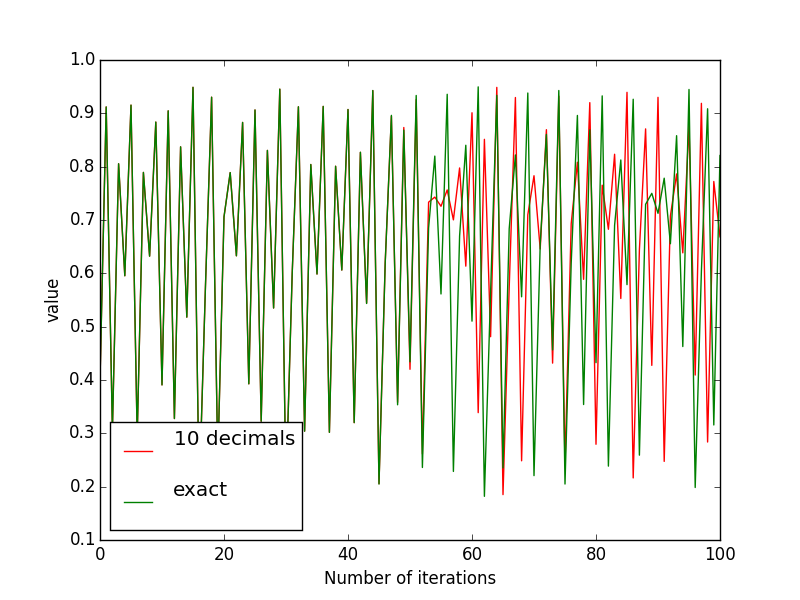
\includegraphics[width=0.5\textwidth]{img/dynamic_systems/logmap1}
    \caption{100 Iterations of the logistic map with $a=3.8$ and $x_0 = 0.4$ computed with 10 decimals precision and exactly.}
    \end{figure}
    \begin{figure}\label{fig:logmapprec}
    \centering
    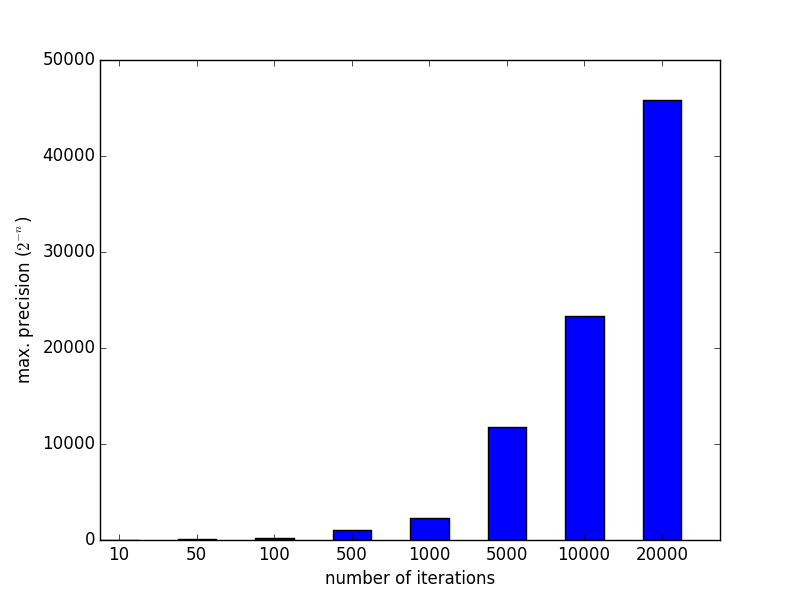
\includegraphics[width=0.5\textwidth]{img/dynamic_systems/logmap2}
    \caption{Maximal precision iRRAM uses to compute iterations of the logistic map and output the points with 10 decimal digits.}
  \end{figure}
  \subsubsection{The Shadowing Lemma}
    The term pseudo-orbit is used to describe numerically generated noisy orbits. 
    \begin{definition}\label{def:pseudoorbit}
      A sequence $(x_i)$ is called an \textbf{$\alpha$-pseudo-orbit} for a map $f$ if
      $ \| x_{i+1} - f(x_i) \| < \alpha $  
    \end{definition}
    One can think of a pseudo orbit as a numerically computed orbit, where small rounding errors can occur in every evaluation of $f$.
    \begin{definition}\label{def:shadowing}
      A real orbit $(y_i)$ \textbf{$\beta$-shadows} the pseudo-orbit $(x_i)$ if 
      $\| x_i - y_i \| < \beta$.  
    \end{definition}
    \begin{definition}
      A dynamic system is called \textbf{uniformly hyperbolic} if ...
    \end{definition}
    For systems that are uniformly hyperbolic Anosov and Bowen could show the following result \cite{anosov1967} \cite{Bowen1975} \cite{Hasselblatt:2008}:
    \begin{theorem}[Shadowing Lemma]
     For all $\beta > 0$ there exists an $\alpha > 0$ so that for every $\alpha$-pseudo-orbit $(x_i)$ there is a point $y_0$ so that the real orbit starting at $y_0$ $\beta$-shadows $(x_i)$.
    \end{theorem} 
    The logistic map is not hyperbolic...\\
    So for non-hyperbolic $f$, it can not be expected, that there is a real orbit that stays close to the pseudo orbit forever.
    Instead, there will be an orbit staying close to $(x_i)$ for some time, say up to some point $n_0$, and then starting to diverge. 
    The goal of this the case study is to investigate such orbits, in particular to find out how long there is an orbit staying close to the pseudo orbit,
    The basis for this case study is a paper by Hammel, Yorke and Grebogi from 1987 \cite{Hammel1987}.
    The paper deals with the question, how long numerical orbits of the logitstic map can be shadowed by true orbits.
    The authors show that for $a = 3.8$ and $x_0 = 0.4$, there is a true orbit $(y_n)$ of the logistic map, so that $\| x_n - y_n \| < 10^{-7}$ for $n \leq 10^7$.
    Their proof method is to compute bounds on the points of the true orbit by using a form of interval arithmetic and letting a computer do the computations. 
    All their computations are done on a Cray X-MP supercomputer. 
    For the case study, first their algorithm was implemented on a modern computer in the \cc programming language, both using fixed precision floating point numbers and \irram. 
    As a second step \irram was used to compute the shadowing orbit exactly.
  \subsubsection{The algorithm}
    The goal of the algorithm is to compute a shadowing orbit $(y_n)$ of size $N$ for a pseudo orbit $(x_n)$ of the logistic map $f$.
    Instead of computing the shadowing orbit from the first point, the algorithm computes the inverse orbit by starting with the last point and then iteratively computing the predecessor. 
    Since the logistic map is not injective, there is not a unique choice for this predecessor. 
    For some point $f(x)$ there are normally two possible values for the inverse given by $f^{-1}_{1,2}(x) = 0.5 \pm \sqrt{0.25 + \frac{x}{a}} $.
    An orbit can be computed by setting $y_N = x_N$ and then iteratively applying one of the inverse map $y_{n-1} = f^{-1}(y_n)$.   To stay close to the pseudo orbit, in every step the point on the same side of $0.5$ as $x_n$ is chosen (the index of $f^{-1}$ will from now on be omitted). 
    This works since the inverse function on $(0,1)$ is a contraction, thus
    $$ \| x_{n-1} - y_{n-1} \| = \| x_{n-1} - f^{-1}(y_n) \| \leq \| f^{-1}(x_n) - f^{-1}{y_n} \| + \| f^{-1}(x_n) - x_{n-1} \| \leq \| x_n - y_n \| + \delta $$   
    Since the original work had to do all the computations using floating point arithmetics, the inverse could not be computed exactly.
    Instead of the points $y_n$, a sequence of intervals $(I_n)$ that bound the location of $y_n$ is computed, i.e. so that $y_n \in I_n \text{ for } 0 \leq n \leq N$.
    The procedure is started with $I_N := [x_n, x_n]$ and then $I_{n-1}$ is selected so that $I_n \subseteq f(I_{n-1})$ holds and $I_n$ is chosen as small as possible. 
    Then the maximal distance between all points in $I_n$ and $x_n$ is computed.
    This gives a shadowing bound.
    An alternative to this algorithm, that instead computes the orbit in forward direction can be found in \cite{chow1991}.
\subsection{Implementation}
  The first part of the case study was to simulate the computations that were made on the Cray X-MP supercomputer on a modern computer. 
  The cray double precision data type used for the computations in the paper has machine epsilon $\varepsilon_\mu = 2^{-95}$.
  To compute the intervals $I_n$ from $I_{n+1}$ the inverse of the interval is computed as described above (using floating point arithmetic).
  Then as long as $I_{n+1} \not \subseteq f(I_n)$, $I_n$ is enlarged on both sides by the minimal possible quantity $\varepsilon_\mu$. 
  Since also the computation of $f(I_n)$ is done using floating point arithmetics, the condition might still not be fulfilled.
  This can, however, be compensated by further enlargening the interval on both sides by the constant $10^{-25}$.
  Since the precision of the clay double data type differs from the IEEE double precision, it was not possible using \cc's built in data types for simulating the algorithm.
  Instead, the boost multiprecision library \cite{boostmultiprecision} was used. 
  The library provides data types that replace the native \cc floating point types, but with a user defined precision. 
  For the interval arithmetic an interval class was implemented, having the following methods:\\
  CLASS DIAGRAM \\
  The same algorithm was also implemented in a different way. 
  Instead of using intervals with fixed precision floating point end points, \irram's \code(INTERVAL) type can be used. 
  The data type provides interval arithmetic for intervals with real numbered end points.
  Then, the inverse of an interval can be computed exactly.
  The next step, was to compute the shadowing orbit exactly.
  For that, only the pseudo orbit was calculated using floating point arithmetics. 
  Then, starting with the last point of the pseudo orbit the inverse was conputed exactly and the distance to the corresponding point in the pseudo orbit calculated.
  The maximum of all those distances is the distance of the shadow orbit and the pseudo orbit.
  One has to be a little careful though, when computing this maximum, since comparing two real numbers is not computable. 
  This problem can, however, easily be solved by the use of multi valued functions. 
\subsection{Evaluation}
  \subsubsection{Comparison with original work}
  The original work mainly deals with the case $a=3.8$ and $x_0 = $.

  Shadowing bound for different parameters
  Breaking point for different precisions
  Real orbit?

  \section{A Data Structure for Analytic Functions}
  \subsection{Introduction}
  \subsection{Representation of Analytic Functions}
  \subsection{Class Overview}
  \subsection{Implementation Details}
  \subsection{Evaluation}
  \subsection{Applications}
  \section{Root Refinement for Real Polynomials}
  \subsection{Introduction}
  \subsection{Implementation}
  \subsection{Evaluation}
  \chapter{Conclusion}
  \section{Future Work}
  \bibliography{thesis}
\end{document}
